\documentclass[xcolor=x11names,compress,11pt]{beamer}
%\documentclass[12pt]{beamer}
\usepackage{tikz}
\usetikzlibrary{decorations.fractals}

\usepackage[utf8x]{inputenc}
\usepackage{ucs}
\usepackage[french]{babel}

\usepackage{amsmath}
\usepackage{amsfonts}
\usepackage{amssymb}

\usepackage{graphicx}
\usepackage{subfigure}
\usepackage{minted}

%% Beamer Layout %%
\useoutertheme[subsection=false,shadow]{miniframes}
\useinnertheme{default}
\usefonttheme{serif}
\usepackage{palatino}
\usepackage{inconsolata}

\setbeamerfont{title like}{shape=\scshape}
\setbeamerfont{frametitle}{shape=\scshape}

\setbeamercolor*{lower separation line head}{bg=DeepSkyBlue4} 
\setbeamercolor*{normal text}{fg=black,bg=white} 
\setbeamercolor*{alerted text}{fg=red} 
\setbeamercolor*{example text}{fg=black} 
\setbeamercolor*{structure}{fg=black} 
 
\setbeamercolor*{palette tertiary}{fg=black,bg=black!10} 
\setbeamercolor*{palette quaternary}{fg=black,bg=black!10} 

\renewcommand{\(}{\begin{columns}}
\renewcommand{\)}{\end{columns}}
\newcommand{\<}[1]{\begin{column}{#1}}
\renewcommand{\>}{\end{column}}
%%%%%%%%%%%%%%%%%%%

\newminted{ocaml}{
  fontsize=\scriptsize
}

\newcommand{\inline}[1]{{\footnotesize \mint{ocaml}@ #1 @}}

%\usetheme{Darmstadt}
%\usetheme{Singapore}

\title[Un moteur physique purement fonctionnel]{
  Implémentation d'un moteur 2D purement fonctionnel
}

\author[A. Guéneau \& D. Nava Saucedo]{
  Armaël Guéneau \& Diégo Nava Saucedo
}

\institute{
  ENS de Lyon \\
  Département d'informatique \\
  L3 - Projet 1 OCaml
}

\date[18/01/2013]{
  {\small 18 janvier 2013} \\
  \vspace{0.8cm}
  \begin{tikzpicture}[decoration=Koch snowflake]
    \draw[DeepSkyBlue4] decorate{ decorate{ decorate{ decorate{ (0,0) -- (3,0) }}}};
  \end{tikzpicture}
%  \vspace{1cm}
%  18 janvier 2013
}

\defbeamertemplate*{footline}{infolines theme}
{
  \hbox{%
    \begin{beamercolorbox}[wd=.25\paperwidth,ht=2.25ex,dp=1ex,center]{author in head/foot}%
      \insertshortauthor
    \end{beamercolorbox}%
    \begin{beamercolorbox}[wd=.54\paperwidth,ht=2.25ex,dp=1ex,center]{title in head/foot}%
      \insertshorttitle
    \end{beamercolorbox}%
    \begin{beamercolorbox}[wd=.13\paperwidth,ht=2.25ex,dp=1ex,center]{date in head/foot}%
      \insertshortdate{}%
    \end{beamercolorbox}%
    \begin{beamercolorbox}[wd=.08\paperwidth,ht=2.25ex,dp=1ex,center]{author in head/foot}%
      \insertframenumber/\inserttotalframenumber
    \end{beamercolorbox}  }%
}

\begin{document}

\begin{frame}
\titlepage
\end{frame}

\begin{frame}
  \frametitle{Introduction}
\begin{exampleblock}{Objectifs :}
  \begin{itemize}
  \item Réalisation d'un moteur physique 2D
  \item Implémentation purement fonctionnelle
  \item Généraliste et réutilisable
  \end{itemize}
\end{exampleblock}
\end{frame}

\begin{frame}
  \frametitle{Plan}
  \tableofcontents
\end{frame}

\section{\scshape Architecture du code}

% La conception architecturale du code du projet participe à son
% caractère généraliste et réutilisable

\subsection*{Utilisation du système de modules d'OCaml}
\begin{frame}
  \frametitle{Architecture du code}
  \framesubtitle{Hiérarchisation et réutilisabilité}
  
  \begin{itemize}
  \item Utilisation du système de modules d'OCaml pour organiser le code.
  \item Pour un module fournissant certaines fonctionnalités :
    abstraction de l'implémentation en définissant sa signature.
  \item Fabriquer un module à partir d'un autre : utilisation de
    \emph{foncteurs}.
  \end{itemize}

\end{frame}

\subsection*{Exemple sur les foncteurs}

\begin{frame}[fragile]
  \frametitle{\small Petit exemple d'utilisation d'un foncteur}

\begin{ocamlcode}
module type OrderedType = sig
  type t
  val compare : t -> t -> bool
end

module Make = functor (M : OrderedType) ->
struct
  type t = M.t list
  let max l = List.fold_left
    (fun max x -> if (M.compare x max) then max else x)
    (List.hd l) (List.tl l)
end

module Int = struct
  type t = int
  let compare = (<)
end

module MaxIntList = Make (Int)
\end{ocamlcode}

\end{frame}

\subsection*{Architecture des modules du projet}
\begin{frame}
  \begin{figure}[h]
    \centering
    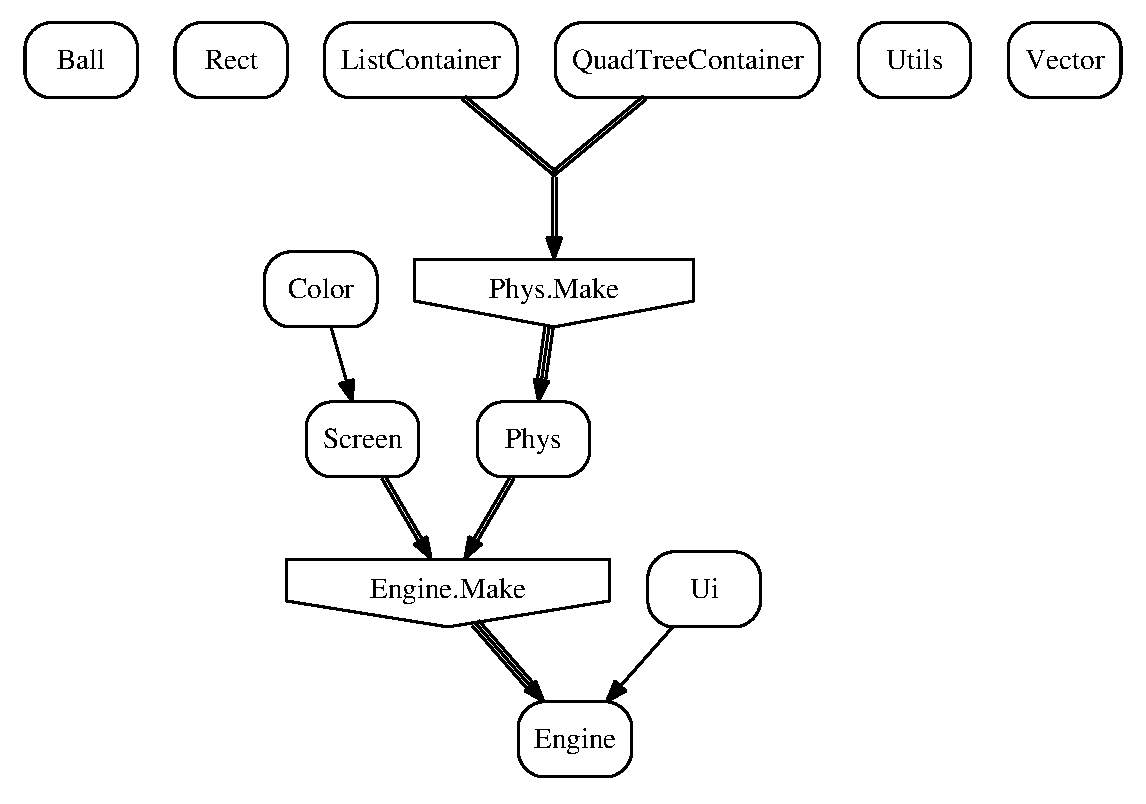
\includegraphics[scale=0.45]{modules.eps}
    \caption{Architecture des modules composant le projet}
  \end{figure}

\end{frame}

\section{\scshape Implémentation fonctionnelle}

\subsection*{Pourquoi ?}

\begin{frame}
\frametitle{Implémentation purement fonctionnelle}
\framesubtitle{\texttt{world >>= change}}

\begin{itemize}
\item Un peu d'originalité !
  \begin{itemize}
  \item Structures de données non mutables
  \item Pas de références
  \end{itemize}
\item Trouver d'autres solutions que celles utilisées dans des codes
  impératifs
\item Lisibilité accrue : pas d'effets de bord de partout sur notre monde
\item Manipulation aisée et performante du monde dans différents états
  \begin{itemize}
  \item Dichotomie temporelle
  \end{itemize}
\end{itemize}

\end{frame}

\subsection*{En pratique}

\begin{frame}[fragile]
\frametitle{\small En pratique}

\begin{itemize}
\item Modification fonctionnelle d'un champ d'un enregistrement
  \begin{ocamlcode}
    {world with height = 300.; width = 200.}
  \end{ocamlcode}
\item Fonctions renvoyant toujours un nouveau \texttt{world}
  \begin{ocamlcode}
    val add_ball : Ball.t -> world -> world
  \end{ocamlcode}
\item Syntaxe agréable pour enchaîner les instructions
  \begin{ocamlcode}
    let ( >>= ) w f = f w

    world >>=
      borders_follow_buffer_size true >>=
      add_f (fun b -> b.mass ** v_down) >>=
      add_random_balls 5. 35. 400. xm ym 70 >>=
      set_restitution 0.9 >>=
      run 60
  \end{ocamlcode}
{\footnotesize
  Le \texttt{world} successivement renvoyé par les différentes
  fonctions est propagé par \texttt{>>=} sans être explicité.}
\end{itemize}

\end{frame}

\section{\scshape Zippers}

\subsection*{Les Zippers}

\begin{frame}
\frametitle{Itérateurs généralistes}
\framesubtitle{Structures de données}

\begin{columns}
\begin{column}[l]{0.35\textwidth}

\begin{figure}[ht]
  \centering
  \raisebox{-0.5\height}{
    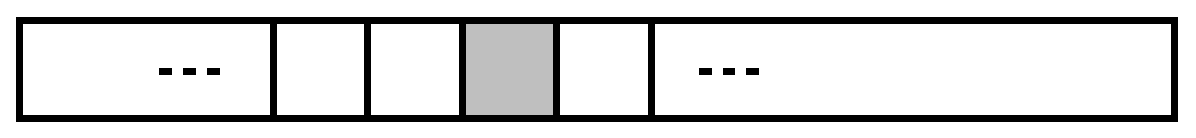
\includegraphics[scale=0.2]{liste.eps}
  }
  \caption{Liste}
\end{figure}

\begin{figure}[ht]
  \centering
  \raisebox{-0.5\height}{
    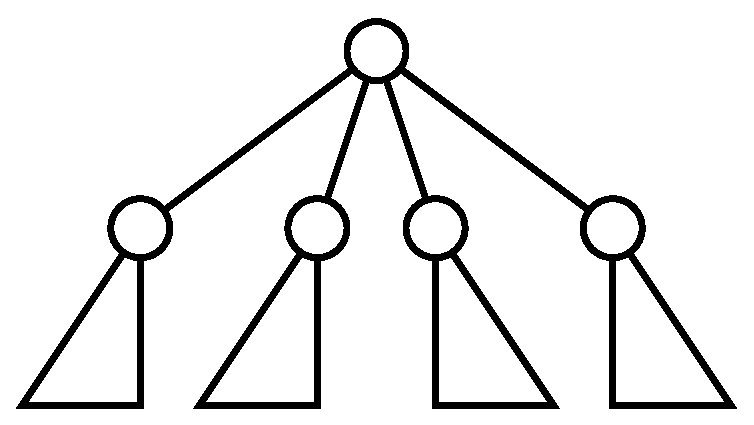
\includegraphics[scale=0.3]{qtree.eps}
  }
  \caption{Quadtree}
\end{figure}
\end{column}

\begin{column}[r]{0.65\textwidth}
  
  \begin{itemize}
  \item Utilisées pour stocker les balles
  \item Liste : toutes les balles sont à la suite
  \item Quadtree
    \begin{itemize}
    \item Nœud : rectangle du plan
    \item Fils : sous-rectangle
    \item On stocke les balles dans les nœuds le plus profondément
      possible sans conflit
    \end{itemize}

  \end{itemize}

\end{column}
\end{columns}

\end{frame}

\subsection*{Problématique}

\begin{frame}
  \frametitle{Itérateurs généralistes}
  \framesubtitle{Problématiques}

  Problème : 
  \begin{itemize}
  \item On a une fonction résolvant la collision entre deux balles.
  \item On veut résoudre toutes les collisions.
  \item Itérer, tout en «~modifiant~» la structure sur laquelle on
    itère.
  \end{itemize}
\end{frame}

\subsection*{Zippers}

\begin{frame}
  \frametitle{Itérateurs généralistes}
  \framesubtitle{Les Zippers}

  \begin{block}{Zipper :}
    Une structure décrivant une \emph{position} dans une autre structure.

    On y associe des fonctions pour déplacer la position et ainsi
    parcourir la structure.
  \end{block}

  \begin{block}{}
    Ils nous serviront d'itérateurs généralistes pour résoudre les
    collisions.
  \end{block}
\end{frame}

\subsection*{Zippers by example}
\begin{frame}[fragile]
\frametitle{Itérateurs généralistes}
\framesubtitle{Les Zippers par l'exemple}

\begin{itemize}
\item Sur les listes :
  \begin{itemize}
  \item \inline{type 'a loc = ('a list) * 'a * ('a list)}
  \item<2-> {\footnotesize \mint{ocaml}@[1;2;3;4;5]@ pos 3
      $\Rightarrow$ \mint{ocaml}@([2;1], 3, [4;5])@ }
  \item<3-> {\footnotesize next : \mint{ocaml}@([3;2;1], 4, [5])@ }
  \end{itemize}
\item<4-> Sur les arbres :
  \begin{itemize}
  \item \inline{type tree = Node of tree * tree | Leaf of int}
  \end{itemize}
\end{itemize}
\end{frame}

\subsection*{Exemple sur les arbres}
\begin{frame}
  \begin{itemize}
  \item \inline{type cxt = Top | L of cxt * tree | R of tree * cxt} 
  \end{itemize}

  \frametitle{\small Exemple sur les arbres binaires}
  \begin{tabular}{|c|l|c|}
    \hline
    $c_0$ & \inline{R (Leaf 1, }$\underbrace{\text{\inline{L (Top, Node (Leaf 3, Leaf 4))}}}_{c_1}$ \inline{)} & %
    \raisebox{-0.5\height}{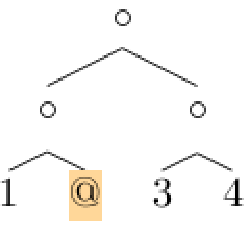
\includegraphics[scale=0.45]{context1.pdf}}\\
    \hline
    $c_1$ & \inline{L (} $\underbrace{\text{\inline{Top}}}_{c_2}$ \inline{, Node (Leaf 3, Leaf 4))} & %
    \raisebox{-0.7\height}{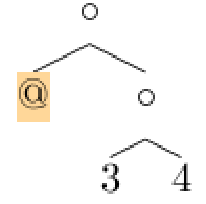
\includegraphics[scale=0.45]{context2.pdf}} \\
    \hline
    $c_2$ & \inline{Top} & \raisebox{-0.2\height}{
\includegraphics[scale=0.45]{context3.pdf}} \\
    \hline
  \end{tabular}

  \uncover<2-> {
    \begin{itemize}
    \item \inline{type loc = cxt * tree}
    \end{itemize}

    \begin{figure}[h]
      \centering
      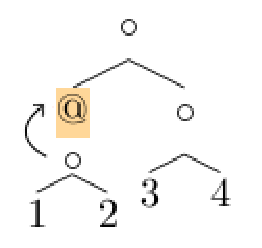
\includegraphics[scale=0.45]{plug_loc.pdf}
    \end{figure}
  }

\end{frame}

\subsection*{Fonctions associées}
\begin{frame}
  Fonctions associées :
  \begin{itemize}
  \item up
  \item left
  \item right
  \item next, effectuant une étape d'un parcours en profondeur
  \item prev, effectuant une étape en sens inverse
  \end{itemize}

\end{frame}

\section{\scshape Gestion de la physique}
\subsection*{Gestion simple sans collisions}
\begin{frame}
\frametitle{Gestion de la physique}
\framesubtitle{Gestion simple sans collisions}

Simulation par intervalles de temps $dt$
\begin{itemize}
\item Simple à mettre en place
\item Robuste
\item Rapide
\item Rendu suffisamment réaliste
\end{itemize}

\uncover<2->{
  Après $dt$, appliquer les forces entrées par l'utilisateur
  \[
  \vec{v} \leftarrow \vec{v} + dt \times \frac{\sum \vec{f}}{m}
  \]\[
  \vec{x} \leftarrow \vec{x} + dt \times \vec{v}
  \]
}
\end{frame}

\subsection*{Gestion des collisions}
\begin{frame}
  \frametitle{Gestion de la physique}
  \framesubtitle{Gestion des collisions}

  \begin{figure}[h]
    \centering
    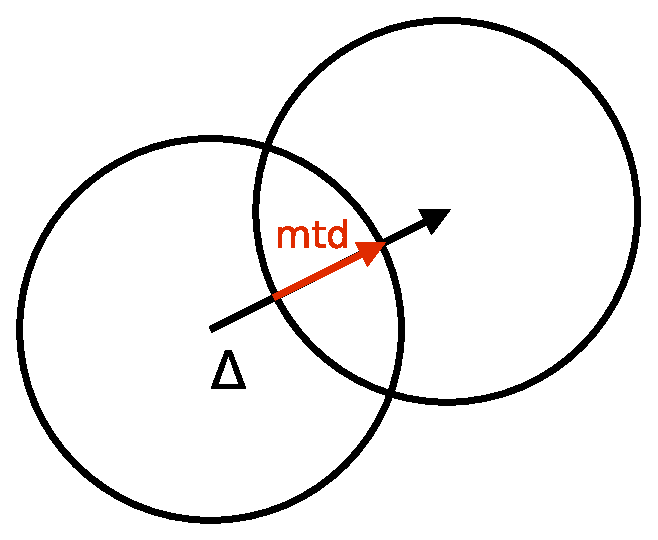
\includegraphics[scale=0.25]{collision.eps}
    \caption{Encastrement après $dt$ devant être résolu}
    
  \end{figure}

  \[
  v_a = \frac{m_a u_a + m_b u_b + m_b C_R (u_b - u_a)}{m_a + m_b}
  \]

  \begin{itemize}
  \item Déplacer les balles selon $\overrightarrow{mtd}$
  \item Calculer les nouvelles vitesses (sur l'axe donné par $\overrightarrow{\Delta}$)
  \end{itemize}

\end{frame}

% Là, on a un moteur physique, utilisant les structures de données
% (conteneurs) purement fonctionnelles d'avant, le moteur est
% encapsulé dans un module autonome (construit à partir du module du
% conteneur)

% Le moteur physique est lui même encapsulé dans un « moteur de jeu »
% qui le relie au module d'affichage et fournit une boucle d'exécution

\section{\scshape Hooks}
\subsection*{Hooks}
\begin{frame}
  \frametitle{Hooks}
  \framesubtitle{Personnaliser et interagir avec le moteur de jeu}

  Participent à la généricité du moteur
  \begin{itemize}
  \item \texttt{predraw\_hook}, \texttt{postdraw\_hook} : fonction
    d'affichage exécutée au début/à la fin du rendu
  \item \texttt{ball\_hook} : fonction personnalisée pour afficher les
    balles
  \item \texttt{user\_action}
    \begin{itemize}
    \item appelé tous les $dt$
    \item reçoit l'entrée utilisateur
    \item peut modifier le monde
    \end{itemize}
  \end{itemize}

  On obtient un moteur de jeu généraliste, réutilisable et hautement
  personnalisable.

\end{frame}

\section{\scshape Applications}
\subsection*{Sandboxes}
\begin{frame}
  \frametitle{Applications}
  \framesubtitle{Simulations physiques}
  \begin{figure}[h]
    \centering
    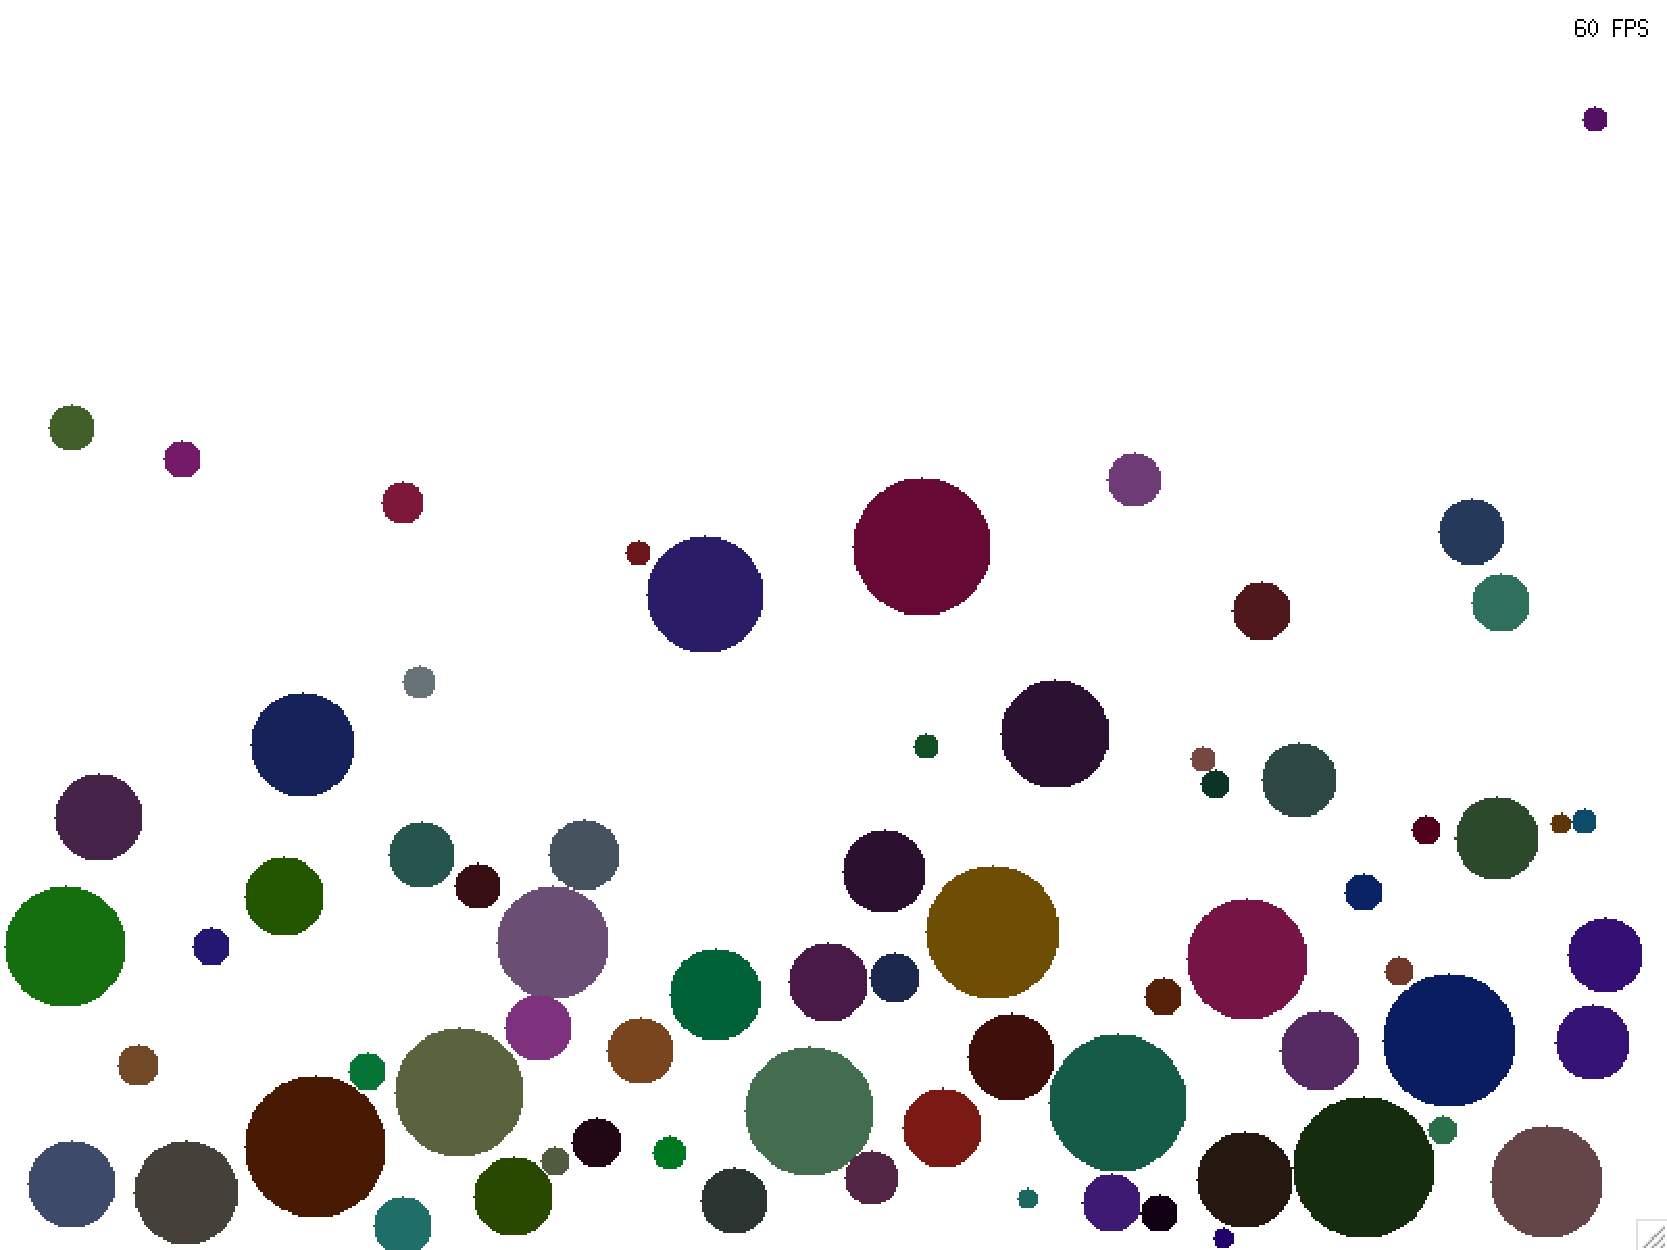
\includegraphics[scale=0.27]{test0.pdf}
    \caption{Gravité et chocs mous}
    
  \end{figure}
\end{frame}

\begin{frame}
  \frametitle{Applications}
  \framesubtitle{Simulations physiques}
  \begin{figure}[h]
    \centering
    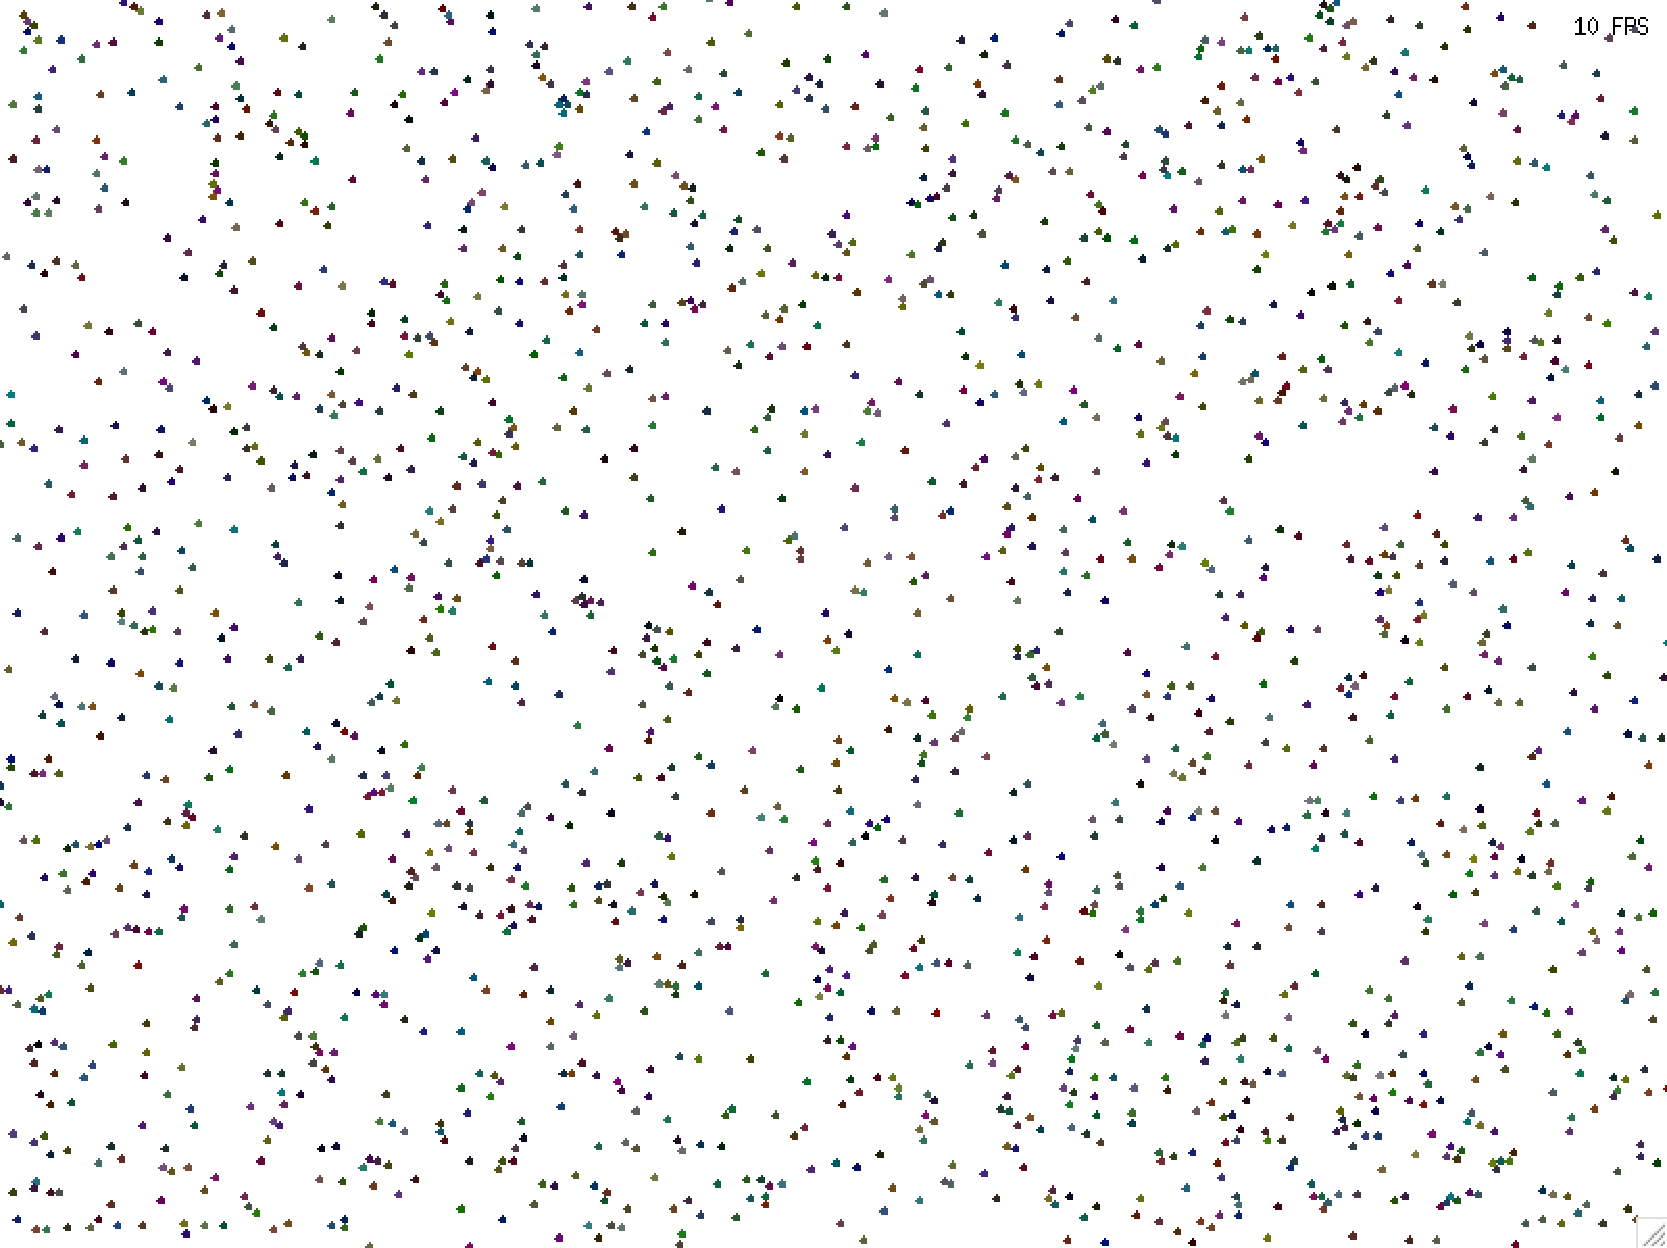
\includegraphics[scale=0.27]{test1.pdf}
    \caption{Pas de gravité, Quadtrees (2000 balles)}
  \end{figure}
\end{frame}

\begin{frame}
  \frametitle{Applications}
  \framesubtitle{Simulations physiques}
  \begin{figure}[h]
    \centering
    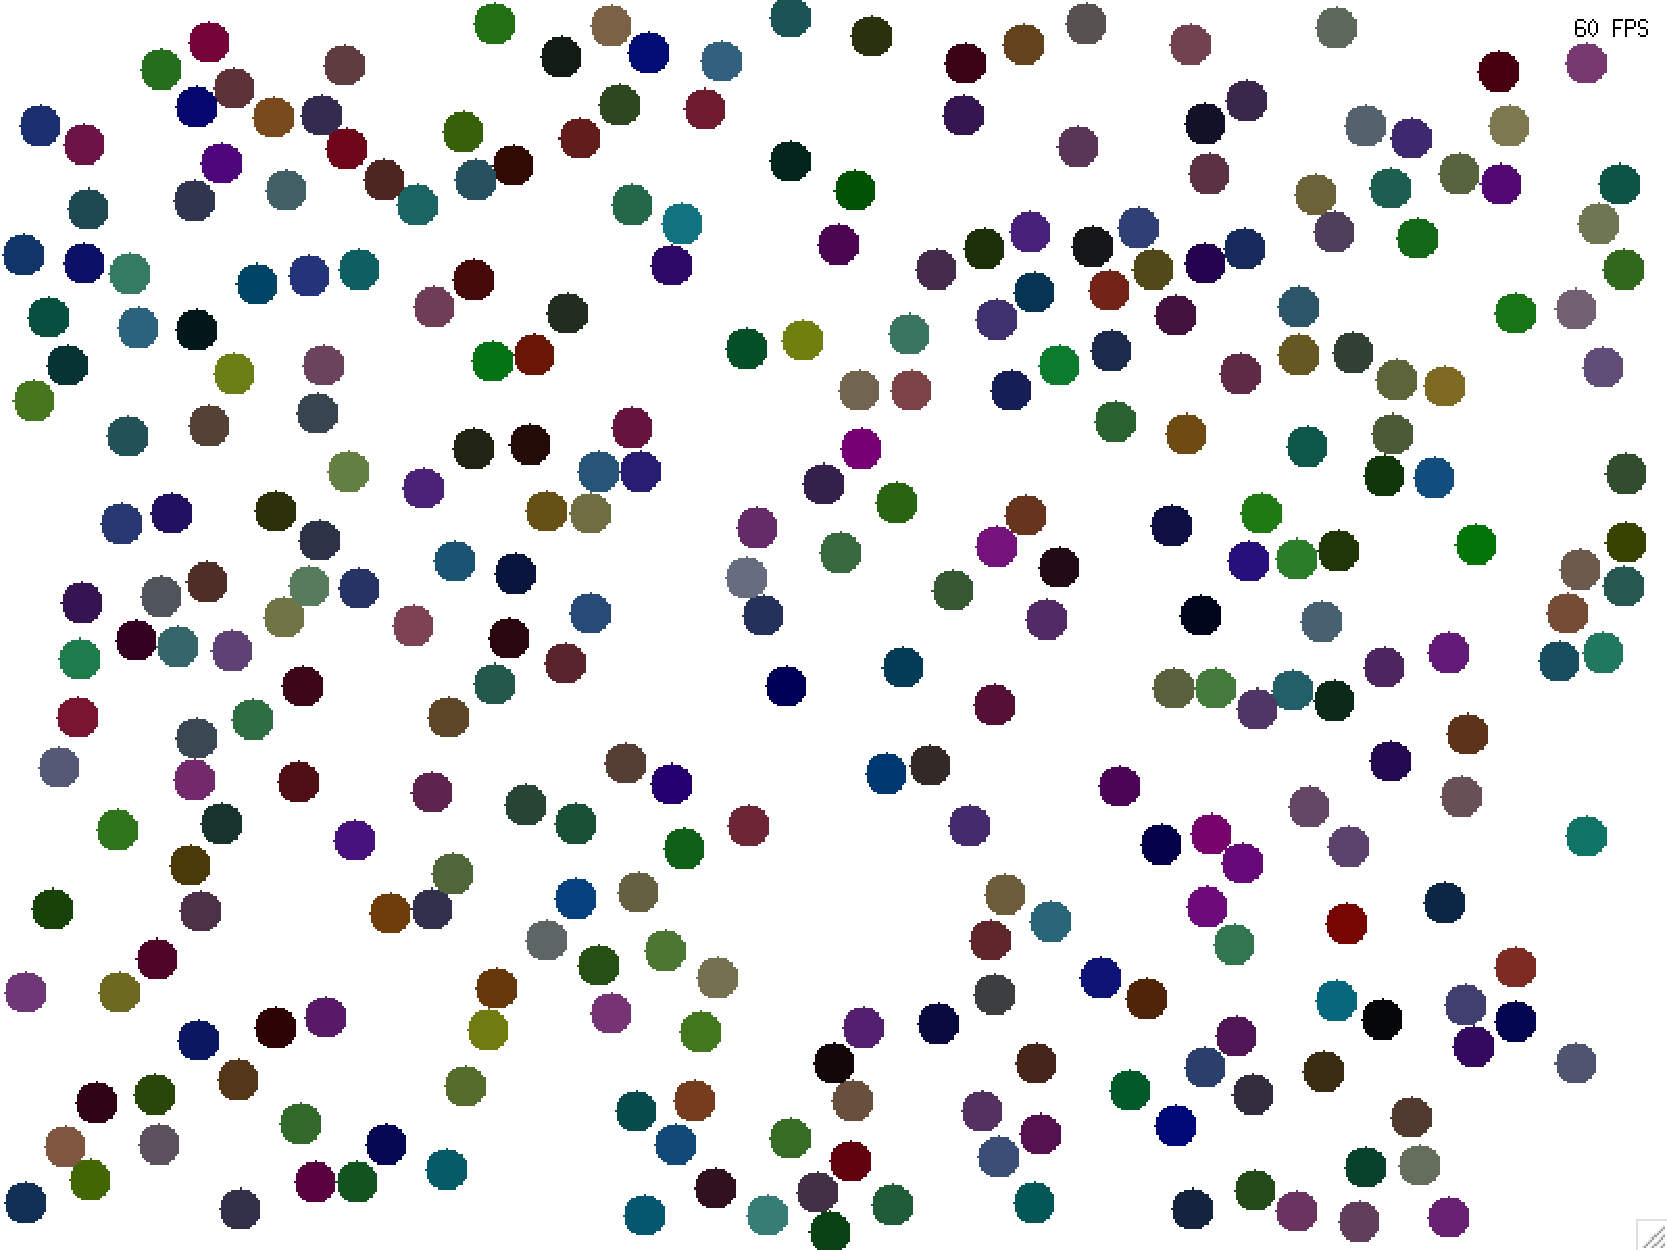
\includegraphics[scale=0.27]{test2.pdf}
    \caption{Situation basique}
  \end{figure}
\end{frame}

\subsection*{Billard}
\begin{frame}
  \frametitle{Applications}
  \framesubtitle{Billard}
  \begin{figure}[h]
    \centering
    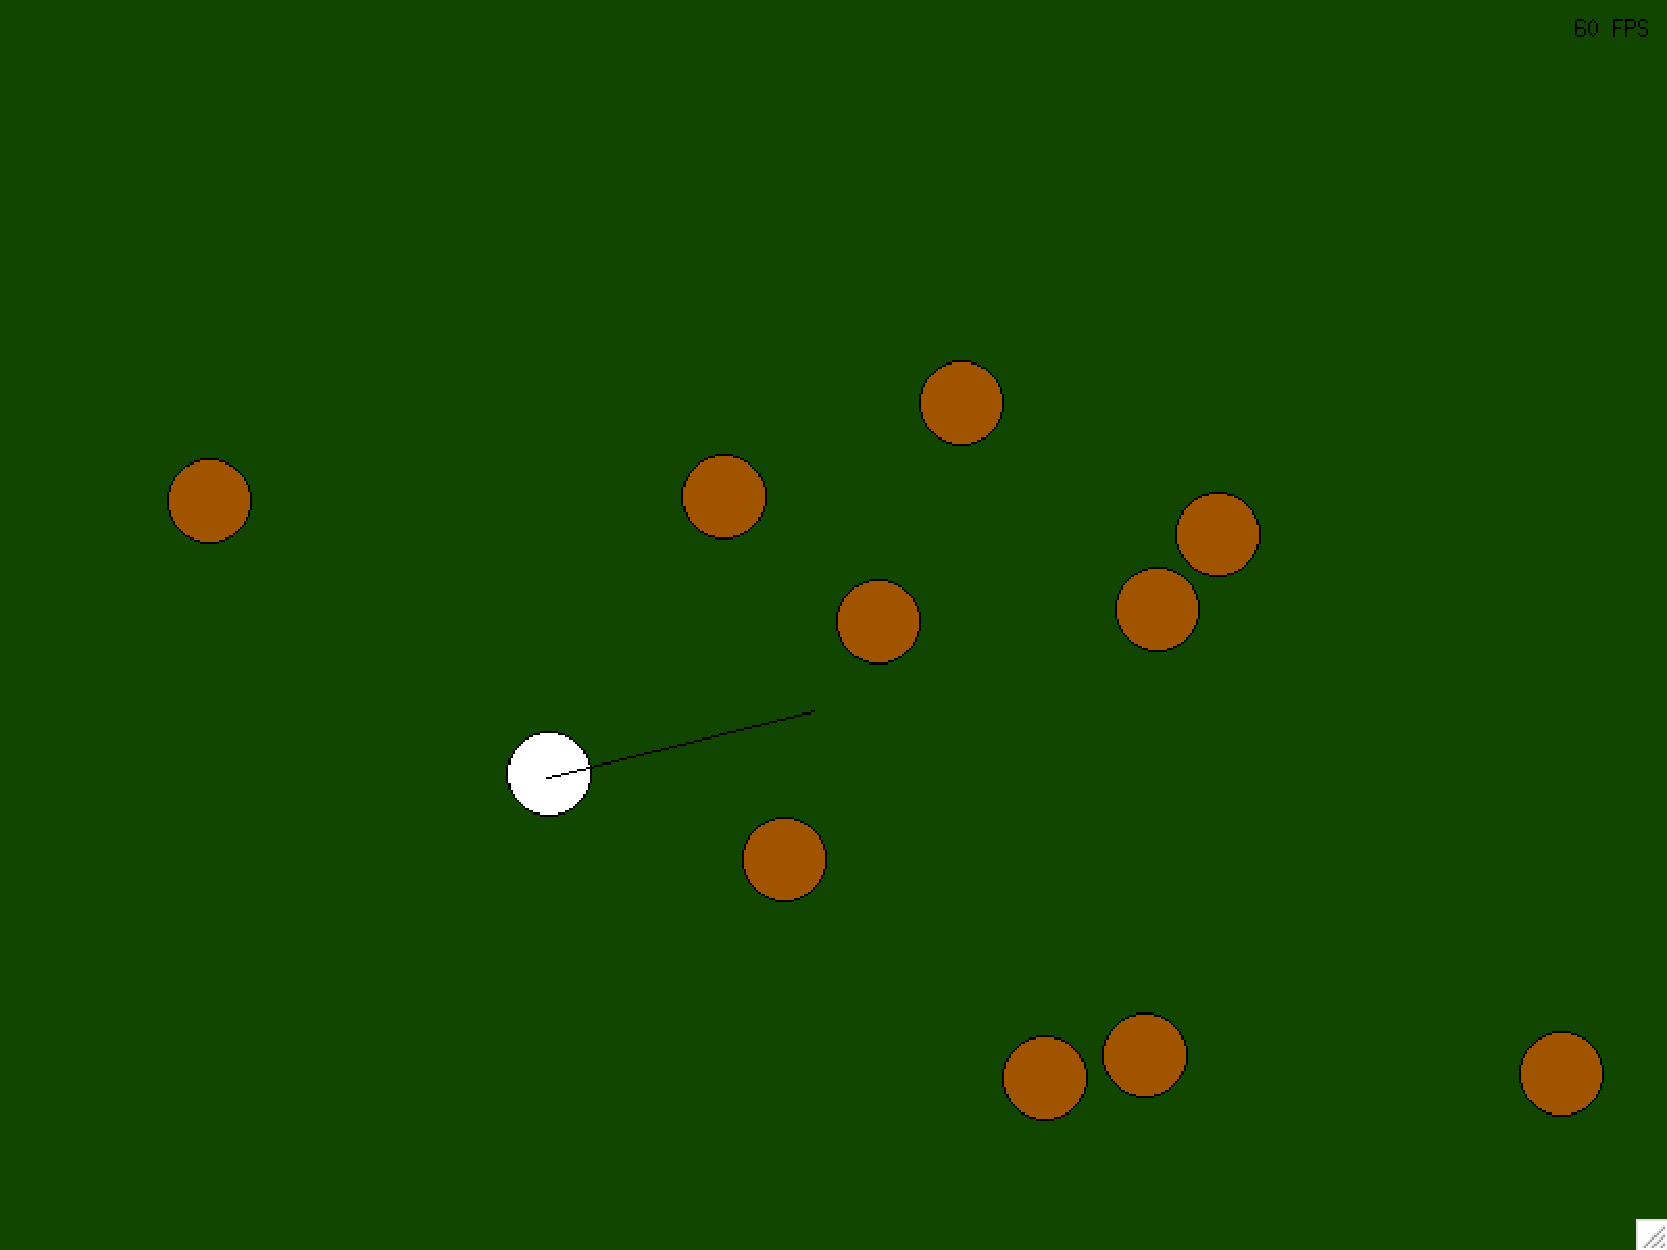
\includegraphics[scale=0.27]{billard.pdf}
    \caption{Billard : gestion de l'entrée utilisateur}
    
  \end{figure}
\end{frame}

\subsection*{MissileCommand}
\begin{frame}
  \frametitle{Applications}
  \framesubtitle{MissileCommand : protégez votre base spatiale !}
  \begin{figure}[h]
    \centering
    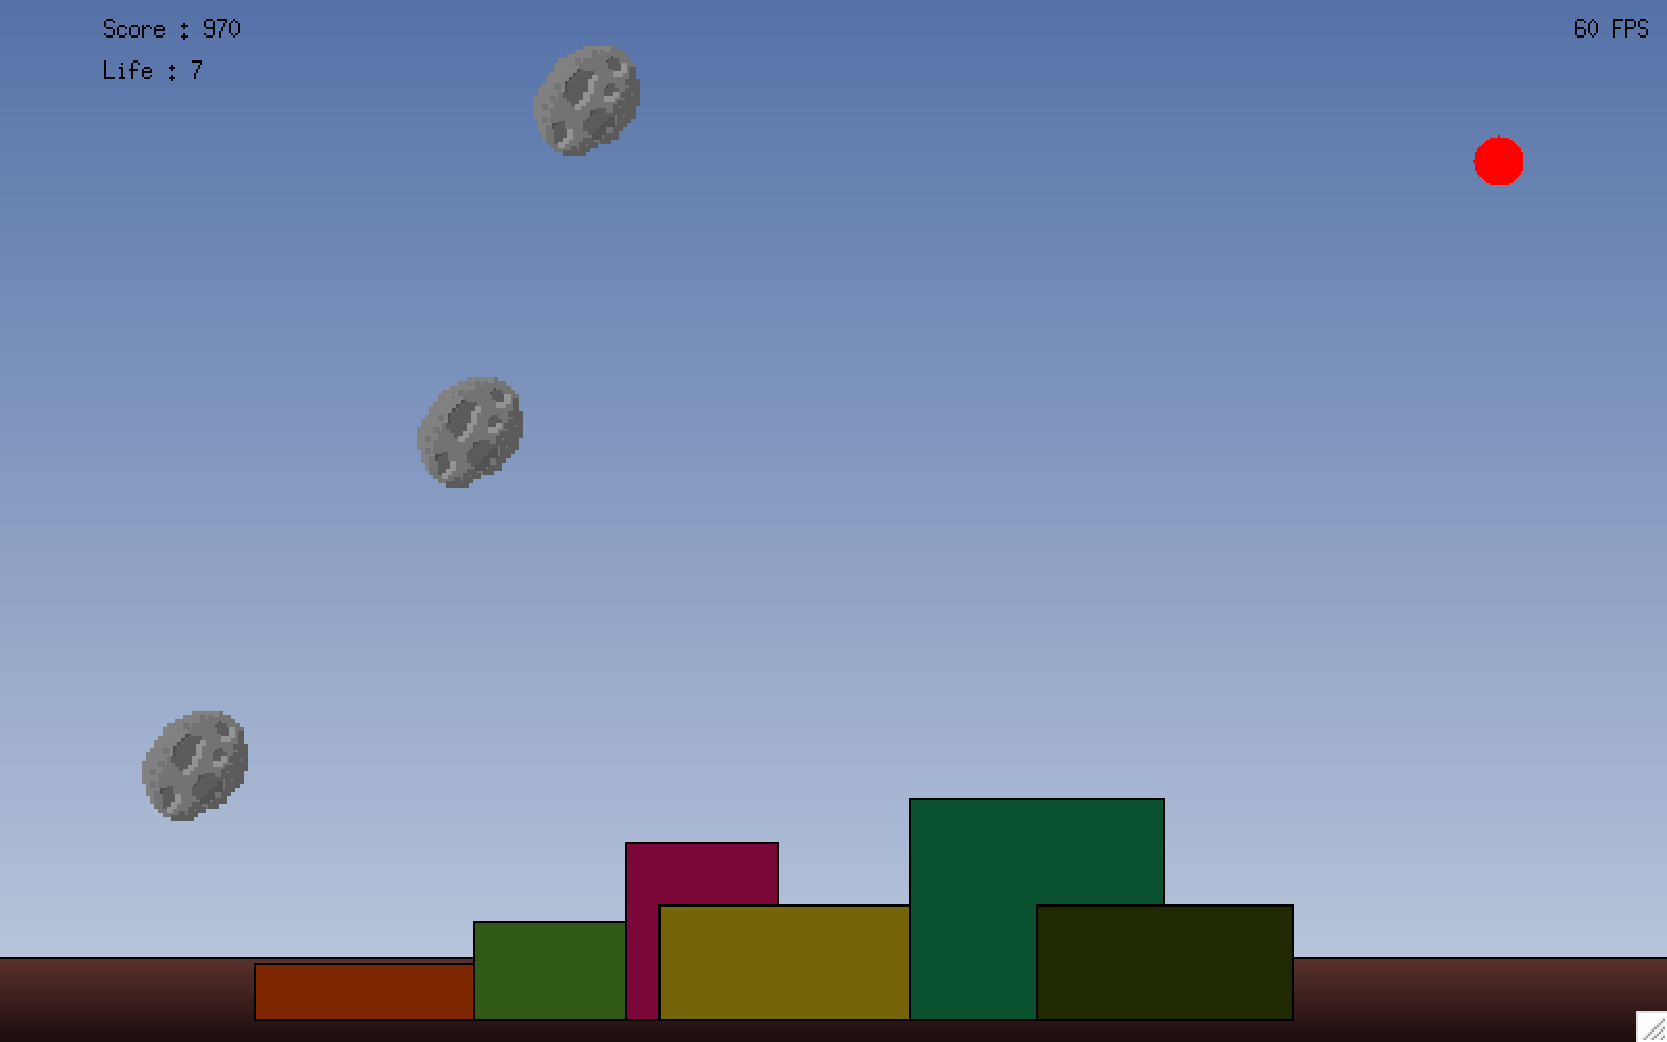
\includegraphics[scale=0.27]{missilecommand.pdf}
    \caption{MissileCommand : fond et balles personnalisées, entrée utilisateur, modification du monde}
  \end{figure}
\end{frame}

\end{document}
